\chapter{Oscilloscope screenshots}

\section{System/Handle plots tab} \label{app:sidetab_ex}
    Here is a screenshot from the tab to create the system and handle plots (\cref{fig:sidetab_ex}).

    \begin{figure}[H]
        \begin{center}
            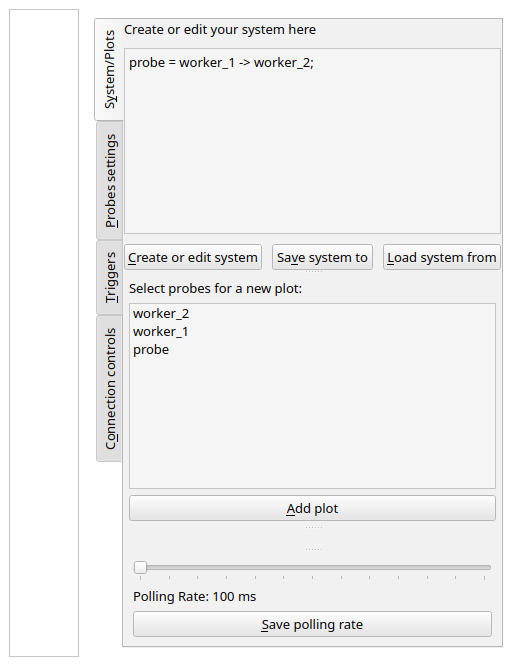
\includegraphics[width = 0.7\textwidth]{img/new_sys_cre.png}
        \end{center}
        \caption{System/Handle plots tab in oscilloscope.}
        \label{fig:sidetab_ex}
    \end{figure}


\section{Parameters tab} \label{app:param_tab}
    Here is a screenshot of the parameters tab, with a set QTA showing up on a plot (\cref{fig:param_tab}).

    \begin{figure}[H]
        \begin{center}
            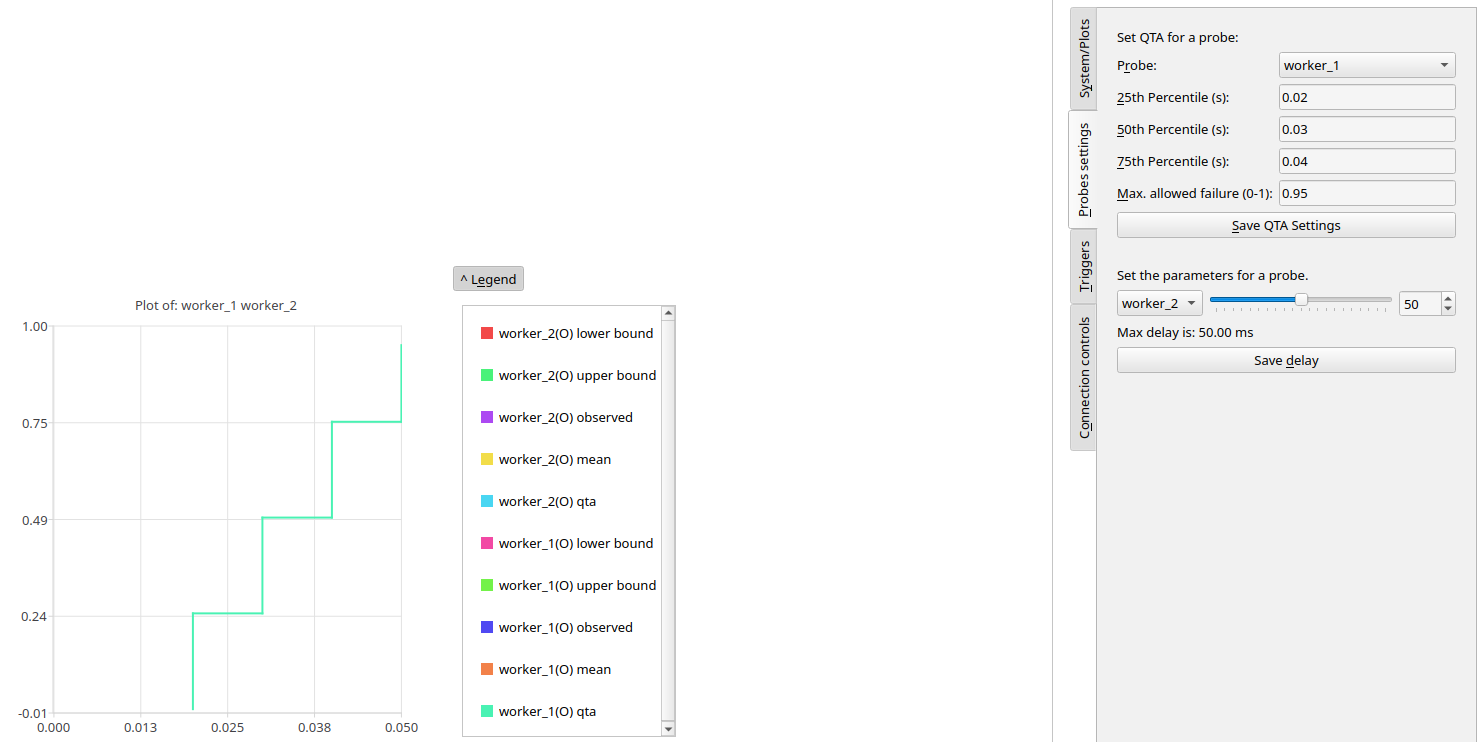
\includegraphics[width = \textwidth]{img/save_qta_manual.png}
        \end{center}
        \caption{Parameters tab in oscilloscope. The QTA set for worker\_1 can be seen on the plot.}
        \label{fig:param_tab}
    \end{figure}

\section{Triggers tab} \label{app:trig_tab}
    Here is a screenshot of the triggers tab, with saved snapshots, QTA violation set for probe and a running plot (\cref{fig:triggers_tab}).

   \begin{figure}[H]
        \begin{center}
            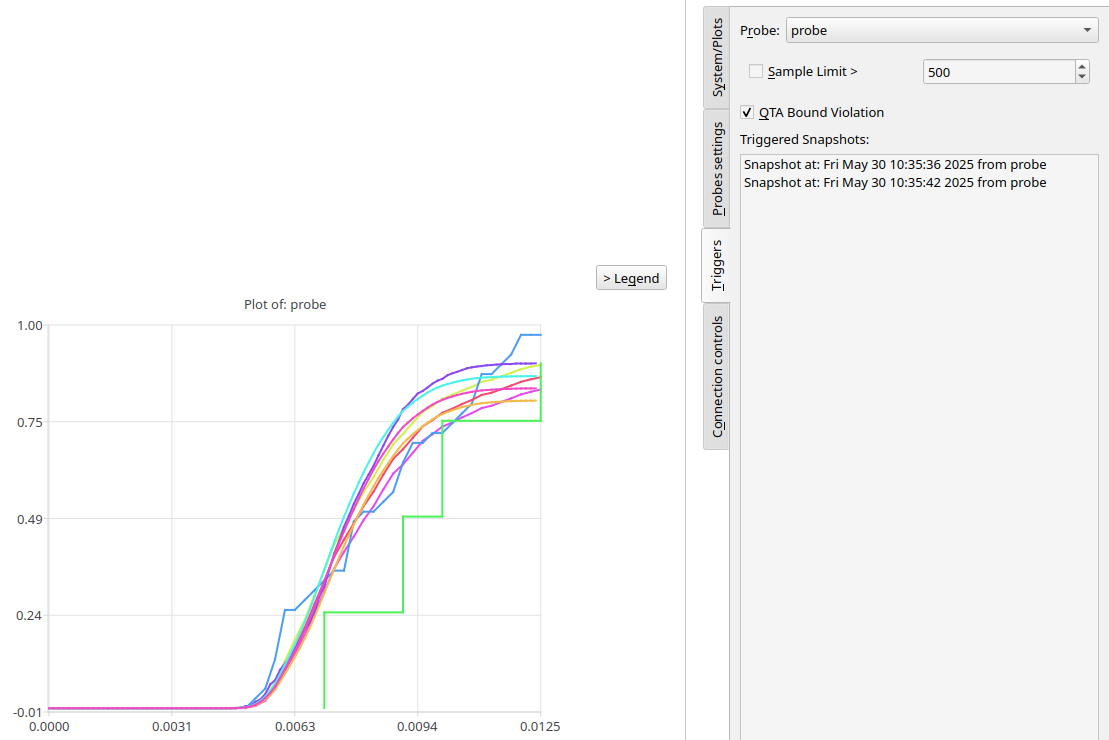
\includegraphics[width = \textwidth]{img/manual/triggers.png}
        \end{center}
        \caption{Triggers tab in oscilloscope. The snapshots for the whole system are saved and can be observed.}
        \label{fig:triggers_tab}
    \end{figure}

\section{Snapshot window} \label{app:snapshot}
    Here is a screenshot from the window observing a snapshot (\cref{fig:control_tab}).

    \begin{figure}[H]
        \begin{center}
            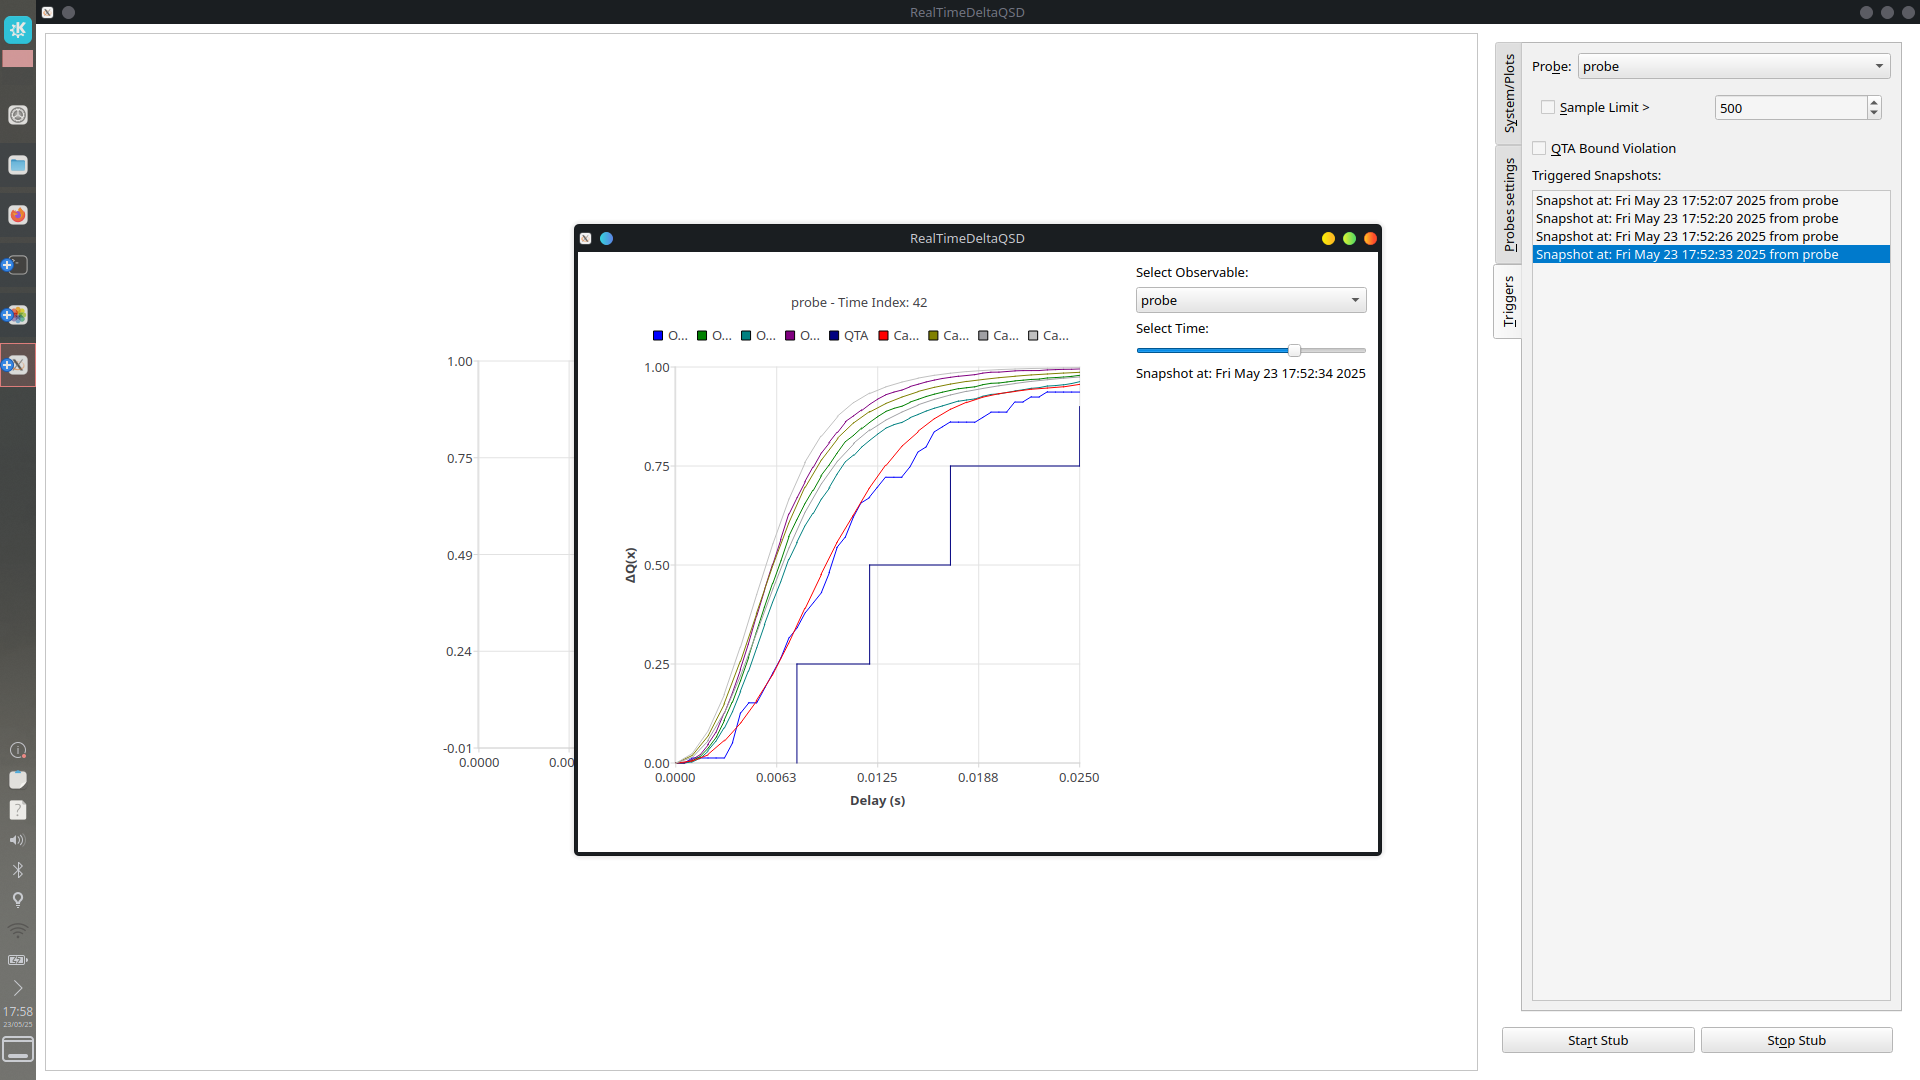
\includegraphics[width = \textwidth]{img/slow_g.png}
        \end{center}
        \caption{Snapshot window (above) over the running oscilloscope below.}
        \label{fig:control_tab} 
    \end{figure}


\section{Connection controls} \label{app:con_control}
    Here is a screenshot of the available controls in the oscilloscope (\cref{fig:control_tab}).
   
   \begin{figure}[H]
        \begin{center}
            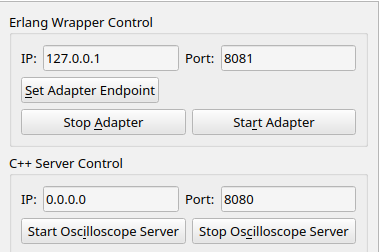
\includegraphics[width = \textwidth]{img/manual/server.png}
        \end{center}
        \caption{Connections control tab in the oscilloscope with the erlang and oscilloscope endpoints.}
        \label{fig:control_tab}
    \end{figure}

\section{Widget view of GUI} \label{app:dash_wid}
    The GUI is composed of multiple building block, the widgets. The screenshot we provide here highlights the multiple widgets present in the GUI (\cref{fig:osc_widgs}). These widgets could be broken down into the multiple subwidgets that compose them.

    \begin{figure}[H]
        \begin{center}
            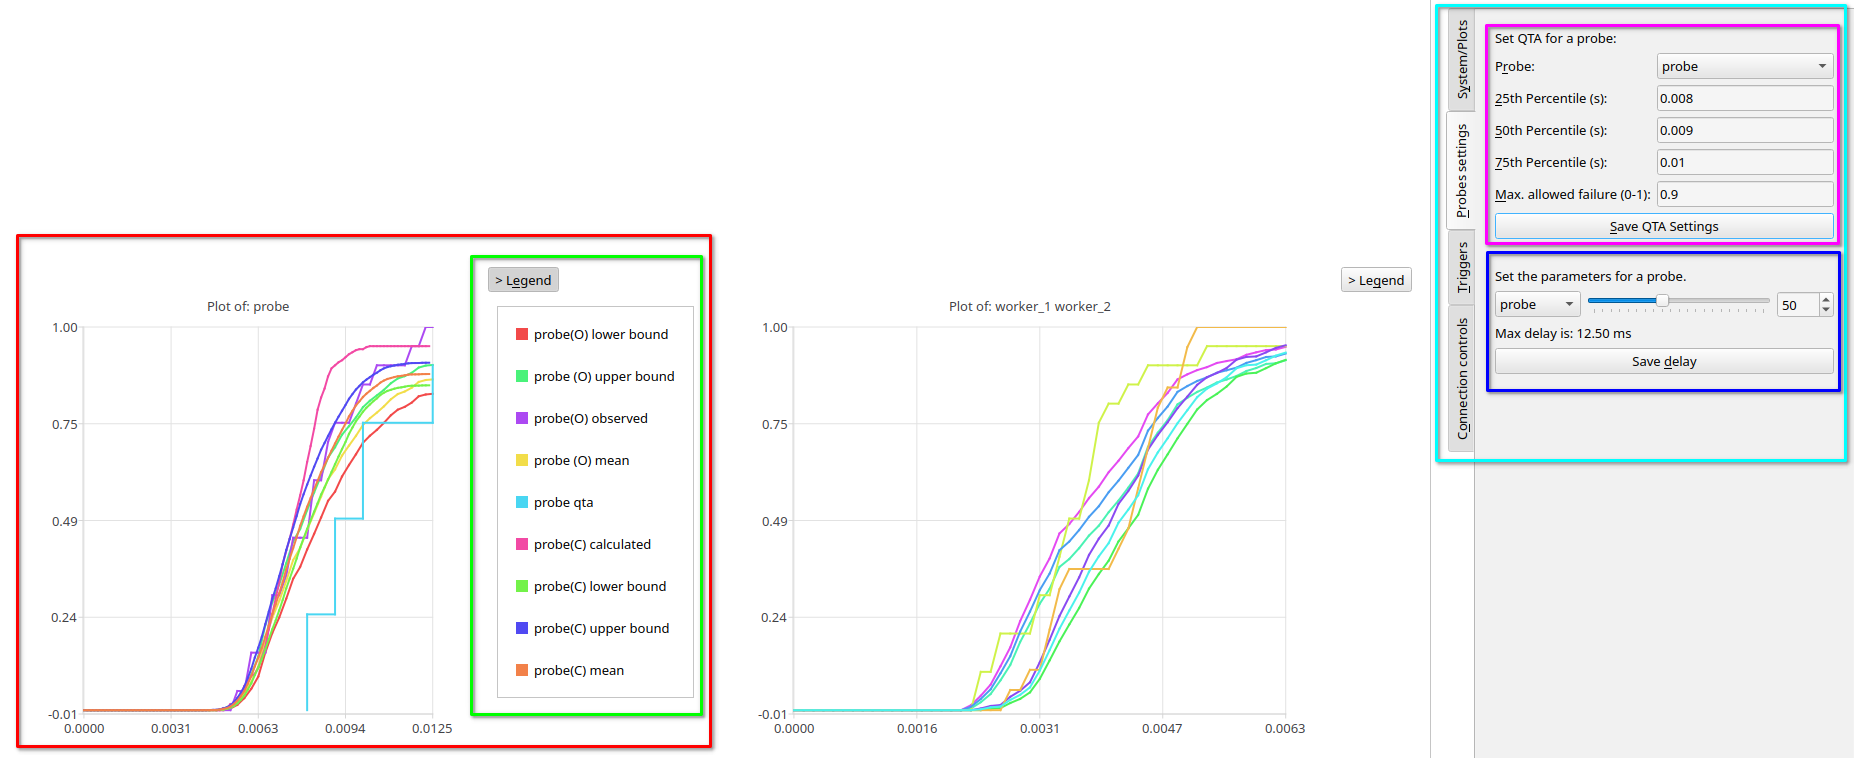
\includegraphics[width = \textwidth]{img/example_osc.png}
        \end{center}
        \caption{Widget view of the oscilloscope dashboard.}
        \label{fig:osc_widgs}
    \end{figure}


